\documentclass[tikz, border=10pt]{standalone}
\usepackage{pgfplots}
\usepackage{amsmath}
\usetikzlibrary{backgrounds}
\pgfplotsset{compat=1.18}

\begin{document}
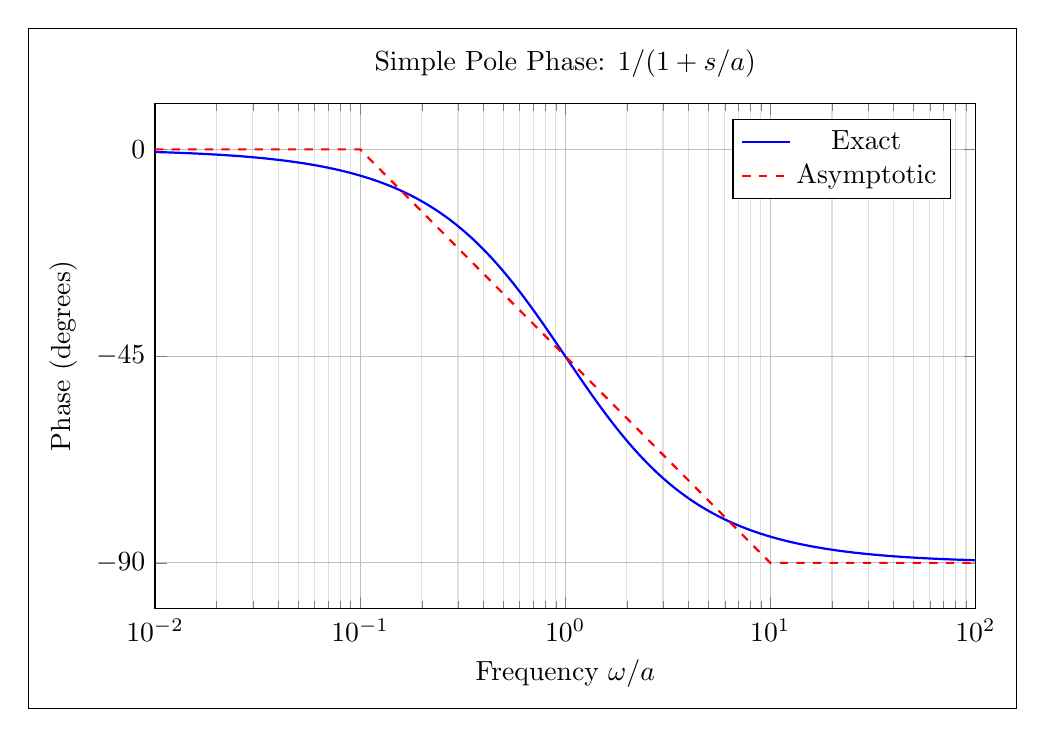
\begin{tikzpicture}[show background rectangle]
    \begin{semilogxaxis}[
        width=12cm, height=8cm,
        title={Simple Pole Phase: $1/(1+s/a)$},
        xlabel={Frequency $\omega/a$},
        ylabel={Phase (degrees)},
        grid=both,
        xmin=0.01, xmax=100,
        ymin=-100, ymax=10,
        minor grid style={gray!25},
        major grid style={gray!50},
        legend pos=north east,
        ytick={0, -45, -90},
    ]

    % Exact: -atan(x)
    \addplot[blue, thick, domain=0.01:100, samples=300] {-atan(x)};
    \addlegendentry{Exact}

    % Asymptotic: 0 < 0.1, -90 > 10
    \addplot[red, dashed, thick] coordinates {
        (0.01, 0) (0.1, 0) (10, -90) (100, -90)
    };
    \addlegendentry{Asymptotic}
    
    \end{semilogxaxis}
\end{tikzpicture}
\end{document}
